\documentclass[sigconf]{acmart}

\usepackage{amsmath}
\usepackage{booktabs}
\usepackage{multirow}
\usepackage{tabularx}
\usepackage{xcolor}
\usepackage{microtype}
\usepackage{pifont}
\setlength{\emergencystretch}{1em}

\AtBeginDocument{\providecommand\BibTeX{{Bib\TeX}}}
\setcopyright{none}
\settopmatter{printacmref=true, printccs=true, printfolios=true}
\renewcommand\footnotetextcopyrightpermission[1]{}
\acmConference[CODS 2026]{ACM India Joint International Conference on Data Science and Management of Data}{December 2026}{India}

% Keep the working benchmark name centralized so that a later rename is safe.
\newcommand{\bench}{\textsc{DoubtBench}}
\newcommand{\pp}{\,pp}
\newcommand{\yes}{\textcolor{green!55!black}{\ding{51}}}
\newcommand{\no}{\textcolor{red!70!black}{\ding{55}}}
\newcommand{\partly}{\textcolor{orange!85!black}{\ding{108}}}
\definecolor{revisionred}{RGB}{190,0,0}
\newcommand{\revision}[1]{\textcolor{revisionred}{#1}}
\newenvironment{revisionblock}{\color{revisionred}}{}
\newcommand{\revisioncaptionsetup}{%
  \captionsetup{labelfont={color=revisionred},textfont={color=revisionred}}}
\newcolumntype{Y}{>{\raggedright\arraybackslash}X}

\begin{document}

\title{\bench: Does Self-Doubt Help Language Models---or Just Make Them Check?}

\author{Anonymous Authors}
\renewcommand{\shortauthors}{Anonymous Authors}

\begin{abstract}
Prompts described as ``emotional'' or ``metacognitive'' frequently combine
self-doubt language with ordinary task directives such as checking an answer,
showing intermediate work, or reconsidering an initial response. A performance
change under such a compound prompt therefore does not identify what caused
the change. We introduce \bench, a paired factorial benchmark for attributing
these prompt effects. The benchmark contains 6,400 procedurally generated
latent tasks spanning eight operational families and 33 task types. Every task
is evaluated under five controlled prompt conditions crossed with two task
contexts, producing ten counterfactual responses for the same model--task
pair. This design separately estimates the effects of pure self-doubt, direct
checking, their combination, output concision, and an existing request for
reasoning. We define the Conditional Doubt Effect (CDE), the incremental
accuracy change from adding self-doubt after checking is already present, as
the primary attribution endpoint, while retaining a decomposed scorecard of
competence, checking gain, context modulation, and robustness. The evaluation
\revision{comprises 423,600 responses from six checkpoints,
four independent foundation families, four task seeds, and held-out surface
forms. CDE ranges from $-1.43$ to $+2.59$ percentage points: three checkpoint
estimates are positive and three are negative. Under minimal requests four of
six checkpoints benefit from doubt beyond checking, but only two do when
reasoning is already requested. Thus self-doubt is not a portable correction
policy; its effect depends on the checkpoint, task family, and existing task
instructions.}
\end{abstract}

\begin{CCSXML}
<ccs2012>
 <concept><concept_id>10010147.10010257</concept_id><concept_desc>Computing methodologies~Machine learning</concept_desc><concept_significance>500</concept_significance></concept>
 <concept><concept_id>10010147.10010178</concept_id><concept_desc>Computing methodologies~Natural language processing</concept_desc><concept_significance>300</concept_significance></concept>
 <concept><concept_id>10002944.10011123.10010912</concept_id><concept_desc>General and reference~Empirical studies</concept_desc><concept_significance>300</concept_significance></concept>
</ccs2012>
\end{CCSXML}
\ccsdesc[500]{Computing methodologies~Machine learning}
\ccsdesc[300]{Computing methodologies~Natural language processing}
\ccsdesc[300]{General and reference~Empirical studies}
\keywords{language-model evaluation, prompting, metacognition, self-doubt, checking, paired experiments}

\maketitle

\section{Introduction}

Consider two instructions: ``You are uncertain about your answer; check your
work carefully'' and ``Check your work carefully.'' If the first improves a
language model's accuracy, did uncertainty help, or did the model simply obey
the checking instruction? This ambiguity is common in work on emotional,
persona, and metacognitive prompting. Prompt labels compress several operative
components---affect, capability claims, self-evaluation, checking, social
stakes, output format, and reasoning requests---into a single treatment.
Comparing that treatment with a neutral baseline can establish that a prompt
has an effect, but cannot attribute the effect to the concept named by its
label.

The distinction matters scientifically and practically. Prior studies report
improvements from emotional stimuli and negative prompts
\cite{li2023emotionprompt,wang2024negativeprompt,zhao2026emotions}, and structured
metacognitive prompting can outperform standard prompting on some language
understanding tasks \cite{wang2024metacognitive}. Yet language models are also
sensitive to apparently incidental prompt choices and output constraints
\cite{sclar2023prompt,tam2024letmespeak}, and
unaided instructions to reflect or reconsider do not reliably correct
reasoning errors \cite{huang2023cannot}. A practitioner therefore cannot infer
from a successful compound prompt that self-doubt is beneficial, nor that the
same wording will transfer to a model or task that already elicits checking.

We formulate this as \emph{metacognitive prompt attribution}. Given a fixed
model and a fixed task, the objective is to determine which controlled prompt
component changes observable task execution. The construct is behavioral: we
do not claim that a model experiences doubt, confidence, or emotion. We ask
whether language describing self-doubt has an incremental effect beyond a
direct instruction to check, and whether that effect changes when the task
already requests visible reasoning.

\begin{figure*}[t]
  \centering
  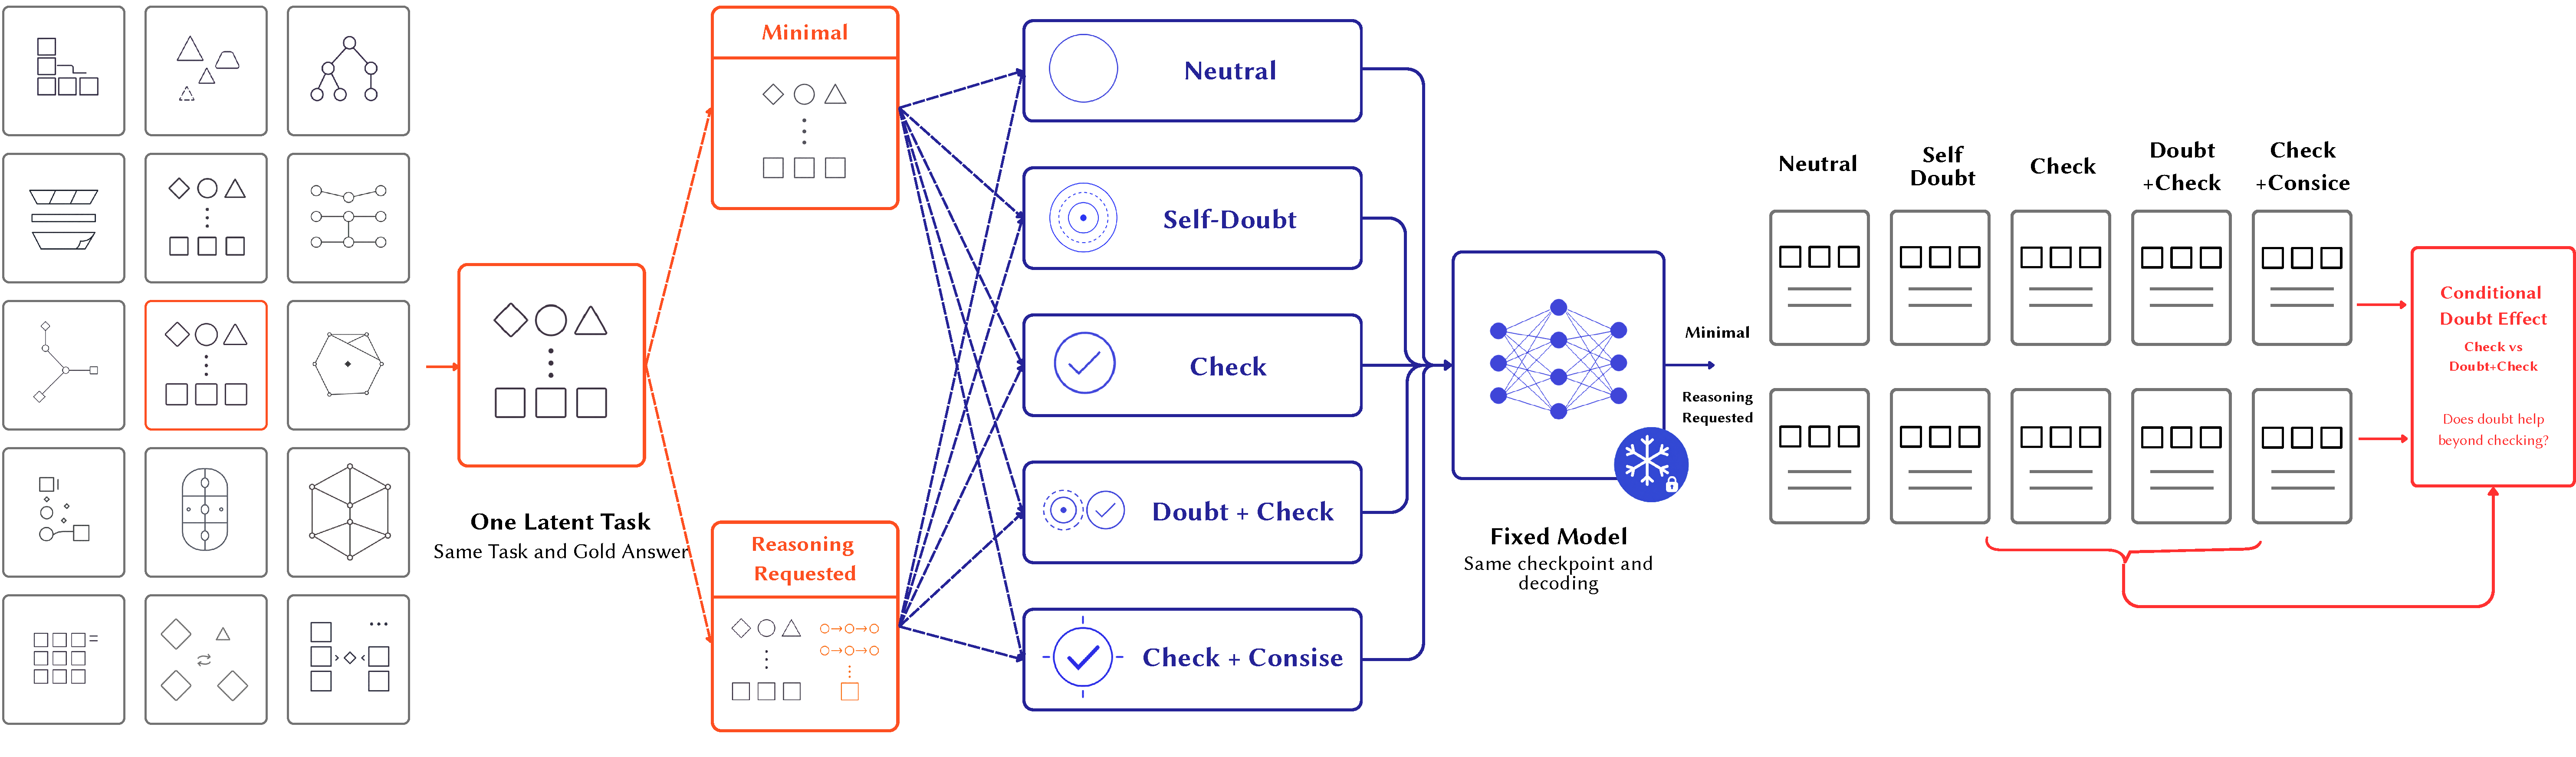
\includegraphics[width=\textwidth]{figures/doubtbench-task-overview.pdf}
  \Description{One deterministic task is crossed with two task contexts and five prompt conditions. A fixed model produces ten paired responses, which are exactly scored to estimate whether self-doubt adds accuracy beyond direct checking.}
  \caption{The \bench{} task. The same latent task and model checkpoint are
  evaluated in all ten factorial cells. Because the neutral, self-doubt,
  checking, combined, and concise conditions share a common prefix and stable
  task ID, the comparison isolates prompt components rather than differences
  in sampled questions.}
  \label{fig:task}
\end{figure*}

We introduce \bench, a benchmark built around this attribution problem
(Figure~\ref{fig:task}). \revision{The benchmark contains 6,400 latent
tasks across eight operational task families and 33 types. Each task has an
exact answer and is crossed with five intervention cells---neutral, pure
self-doubt, direct checking, self-doubt plus checking, and checking plus
concision---and two task contexts: minimal and reasoning-requested. The key
comparison is not self-doubt versus neutral. It is self-doubt plus checking
versus checking alone, which estimates whether doubt contributes after the
ordinary behavioral directive has been held fixed.}

This formulation differs from both general reasoning benchmarks and existing
metacognitive evaluations. General benchmarks rank models by correctness but
do not identify why a prompt changes that correctness. Calibration benchmarks
test whether models know when they are likely to fail
\cite{wang2026mirror}; sycophancy benchmarks test whether a model changes its
answer after a user expresses doubt or supplies a correction
\cite{sinha2026sycobench}. \bench{} instead intervenes before the answer,
separates self-directed doubt from checking language, and crosses those
components with instructions already present in the task.

Our contributions are:
\begin{itemize}
  \item \textbf{A task and benchmark.} We define metacognitive prompt
  attribution and provide a procedurally generated benchmark with
  exact scoring, controlled difficulty, independent task seeds, and held-out
  surface forms.
  \item \textbf{A paired factorial design.} Five prompt cells crossed with two
  task contexts distinguish self-doubt, checking, visible reasoning, and
  concision while keeping the underlying task fixed.
  \item \textbf{A headline endpoint and decomposed scorecard.} The Conditional
  Doubt Effect measures self-doubt beyond checking; companion metrics retain
  baseline competence, checking gain, context modulation, and robustness
  rather than hiding them inside an arbitrary scalar.
  \item \revision{\textbf{A cross-model empirical study.} Across six
  checkpoints from four independent foundation families, CDE is split evenly
  between positive and negative estimates and changes sharply with task
  context. The study further isolates task-family, seed, surface-form, and
  within-lineage post-training heterogeneity.}
\end{itemize}

\section{Related Work and Benchmark Positioning}

\paragraph{Emotional and negative prompting.}
EmotionPrompt studies psychologically inspired stimuli appended to prompts
\cite{li2023emotionprompt}; NegativePrompt focuses on negative emotional
stimuli \cite{wang2024negativeprompt}. These interventions are useful evidence
that prompt semantics can change model behavior. Broader cross-model evidence
also suggests that emotional framing is task- and model-dependent
\cite{zhao2026emotions}. These studies aim to measure or improve aggregate
performance, not to separate self-doubt from an embedded checking instruction
under a common-prefix factorial.

\paragraph{Metacognitive prompting and self-correction.}
Metacognitive Prompting structures a response into interpretation, preliminary
judgment, critical evaluation, final decision, and confidence
\cite{wang2024metacognitive}. Chain-of-thought and related scaffolds can elicit
additional reasoning \cite{wei2022chain}, but reflection without external
feedback is not a dependable correction mechanism
\cite{huang2023cannot}. Iterative systems such as Self-Refine instead add an
explicit feedback-and-revision loop \cite{madaan2023selfrefine}; that is a
different intervention from a one-shot pre-answer self-doubt clause. Our
question is prior to method optimization: when a metacognitive-looking prompt
helps, which textual component deserves credit?

\paragraph{Metacognition, calibration, and social pressure.}
MIRROR evaluates self-knowledge and the transition from monitoring to action
across multiple metacognitive levels \cite{wang2026mirror}. Earlier work also
finds that models can often estimate whether their own answers are correct
\cite{kadavath2022mostly}. SycoBench-600
measures robustness and selective correction after user doubt, authority, or a
suggested answer \cite{sinha2026sycobench}, extending a broader line of
model-written evaluations that exposed sycophantic agreement with user views
\cite{perez2022modelwritten}. These are complementary problems.
\bench{} neither treats verbal confidence as an internal state nor introduces
post-answer social pressure. It tests pre-answer prompt components on the same
latent task.

\paragraph{Prompt sensitivity.}
Prompt formatting and perturbation studies demonstrate that evaluations can be
brittle to wording and response constraints
\cite{sclar2023prompt,tam2024letmespeak}. Some measured sensitivity can also be
an artifact of the evaluation heuristic rather than a change in task
competence \cite{hua2025flaw}. \bench{} therefore uses task-specific exact
parsers, reports parse failures separately, keeps a shared prompt prefix, and
tests whether the estimated effect survives answer-preserving surface changes.

\begin{table*}[t]
\centering
\caption{Positioning against representative evaluation paradigms. A checkmark
means the property is central and explicit; a circle denotes partial coverage.
The columns concern attribution design, not the overall quality or scope of the
referenced work. ``Context cross'' means that prompt components are factorially
crossed with task instructions that may already elicit the target behavior.}
\label{tab:positioning}
\small
\begin{tabularx}{\textwidth}{@{}Yccccc@{}}
\toprule
\textbf{Evaluation} & \textbf{Component audit} & \textbf{Doubt/check split} & \textbf{Context cross} & \textbf{Exact paired outcomes} & \textbf{Fresh procedural tasks} \\
\midrule
EmotionPrompt \cite{li2023emotionprompt} & \no & \no & \no & \partly & \no \\
NegativePrompt \cite{wang2024negativeprompt} & \no & \no & \no & \partly & \no \\
Metacognitive Prompting \cite{wang2024metacognitive} & \no & \no & \no & \partly & \no \\
Prompt-sensitivity evaluation \cite{sclar2023prompt} & \partly & \no & \no & \yes & \no \\
MIRROR \cite{wang2026mirror} & \partly & \no & \no & \yes & \revision{\ding{108}} \\
SycoBench-600 \cite{sinha2026sycobench} & \partly & \no & \no & \yes & \revision{\ding{55}} \\
\midrule
\textbf{\bench{} (ours)} & \yes & \yes & \yes & \yes & \yes \\
\bottomrule
\end{tabularx}
\end{table*}

\section{\bench}
\label{sec:benchmark}

\subsection{Task Formulation}

A latent task instance is a tuple
$x=(u,g,a,f,d,s)$ containing rendered task instructions $u$, hidden generator
state $g$, gold answer $a$, task family $f$, difficulty $d$, and split seed
$s$. Evaluated models receive only $u$ and the applicable prompt condition;
they never receive $g$, the answer derivation, or scorer metadata. The answer
space may be an integer, label, ordered sequence, set, short symbolic string,
or constrained action plan. Every type has a deterministic parser and scorer.

For a fixed model checkpoint $m$, task $x_i$, prompt condition $c$, and task
context $t$, the evaluation produces one response
$r_{mict}$. The same $i$ appears in every factorial cell. This makes the task
ID, rather than an independently sampled question, the unit of pairing. A model
is not compared with a different model on a different subset to infer a prompt
effect.

The benchmark operationalizes \emph{prompt-induced cognitive-control
behavior}: changes in exact task execution under controlled prompt
interventions. The task families require transient state maintenance,
distractor inhibition, rule switching, error monitoring, relational
integration, and goal management. These labels describe computational task
requirements; they do not assert psychometric equivalence to human clinical or
neuropsychological tests. The design follows the behavioral-testing tradition
of capability-specific, templated tests \cite{ribeiro2020checklist}, extended
by controlled synthetic generation and validation \cite{zhao2024syntheval}.

\subsection{Hidden-Answer-First Construction}

Benchmark generation begins with human-authored task schemas, not free-form
question generation. Each schema specifies admissible latent values,
difficulty parameters, rendering constraints, an answer function, and a
parser. A seeded generator first samples the latent state, computes the exact
answer, and only then renders the instructions. Thus surface text cannot
silently redefine the answer key.

\begin{figure*}[t]
  \centering
  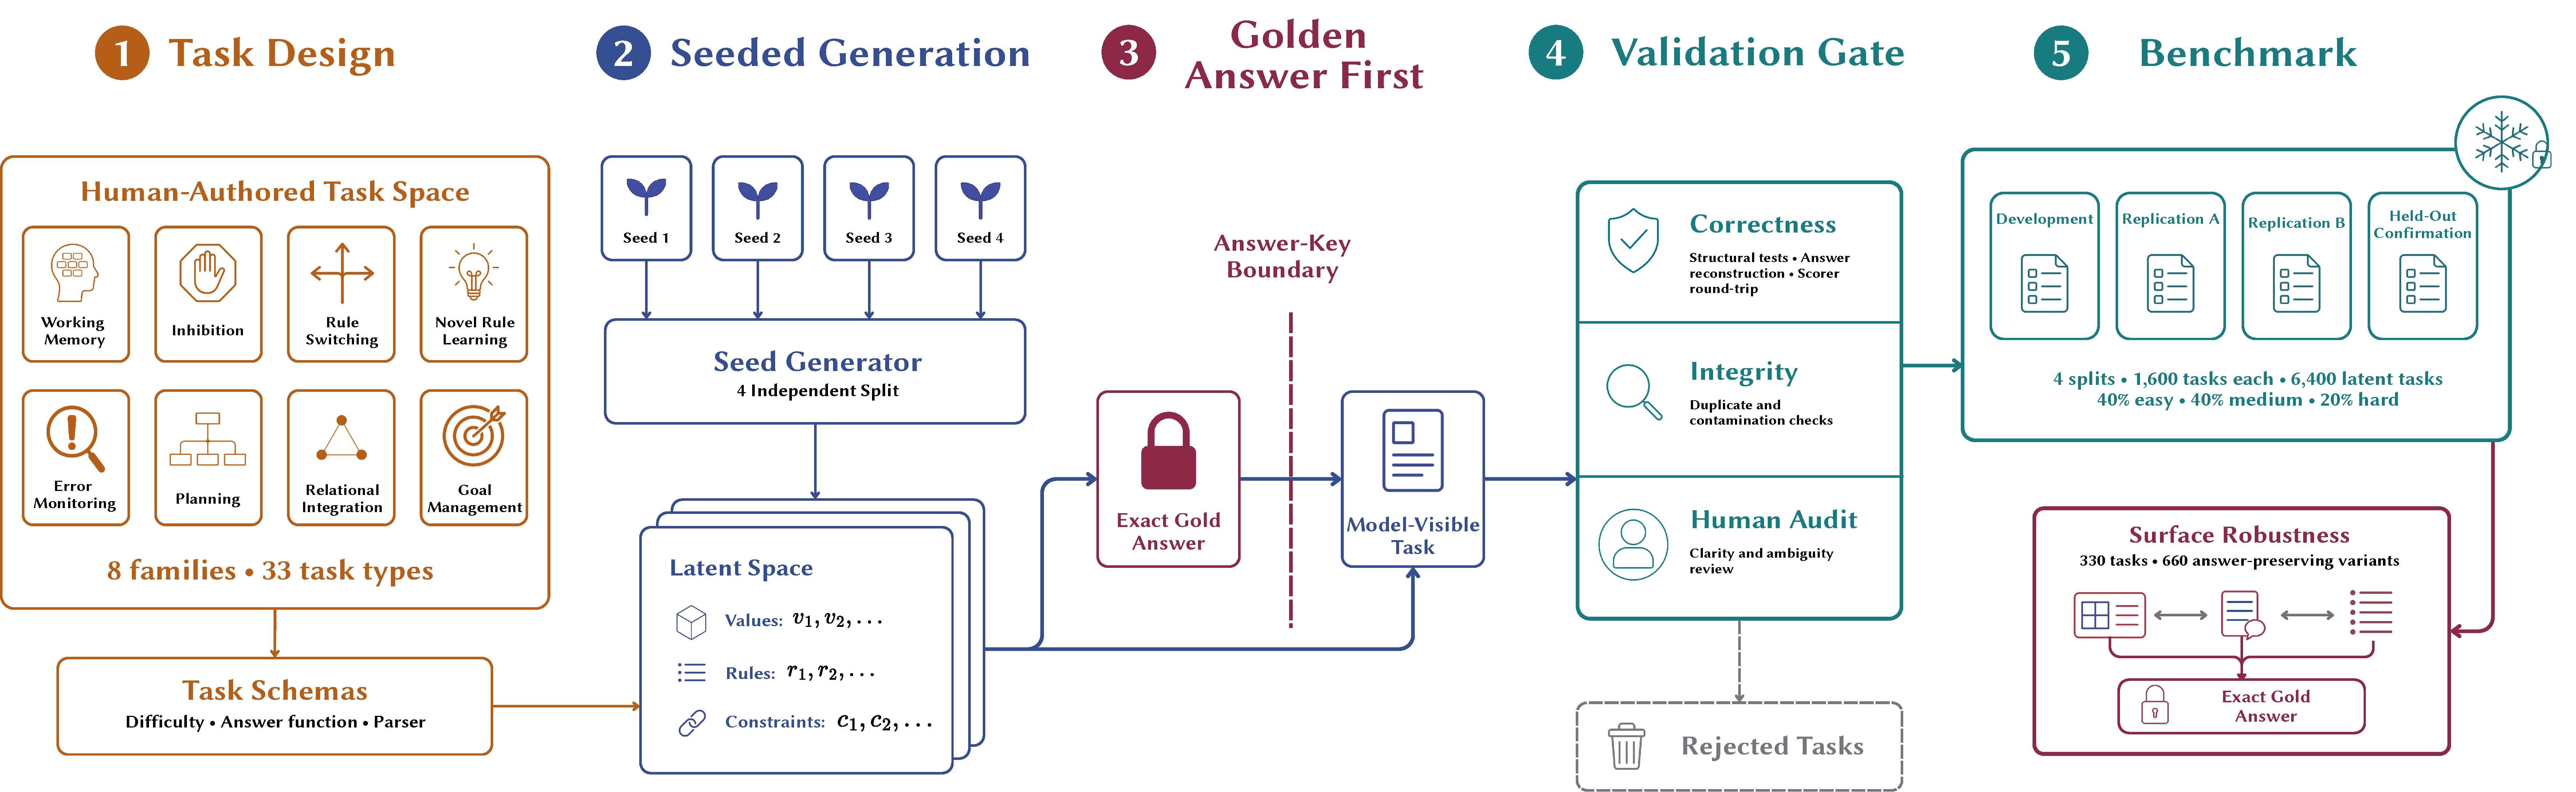
\includegraphics[width=\textwidth]{figures/doubtbench-construction.pdf}
  \revisioncaptionsetup
  \Description{Human-authored task controls feed deterministic task generation, independent validation, a four-split benchmark, and finally the paired prompt factorial. Gold derivations remain behind the answer-key boundary.}
  \caption{\revision{\bench{} construction. Human-authored controls define the task
  space; seeded programs generate latent instances and exact answers;
  independent checks validate the benchmark; and only then are tasks
  crossed with prompt conditions. The model never observes generator state or
  answer-key metadata. The four splits are independent generator replications,
  not training, validation, and test partitions.}}
  \label{fig:construction}
\end{figure*}

Figure~\ref{fig:construction} separates three boundaries that are often
blurred in synthetic evaluation. First, benchmark authors determine the
construct and task schemas. Second, deterministic generators instantiate those
schemas without consulting evaluated model outputs. Third, prompts and model
responses are frozen only after task/scorer validation. \revision{The held-out
seed is reserved before evaluation and is not used to revise task templates,
prompt wording, thresholds, or scorers after responses are inspected.}

\subsection{Task Families and Scale}

\revision{\bench{} contains eight families and 33 task types}
(Table~\ref{tab:families}). Each of four independent splits contains 200 tasks
per family, for 1,600 tasks per split and 6,400 latent tasks overall. Within
each family, the allocation is 40\% easy, 40\% medium, and 20\% hard. Task
types are distributed as evenly as possible inside the family so that a family
score cannot be dominated by one high-volume template.

\begin{table*}[t]
\centering
\revisioncaptionsetup
\caption{\revision{\bench{} inventory. Counts refer to distinct latent
tasks before crossing prompts or task contexts. Every family contributes 200
tasks to each split and 800 across four splits.}}
\label{tab:families}
\small
\begin{tabularx}{\textwidth}{@{}YcYrr@{}}
\toprule
\textbf{Family} & \textbf{Types} & \textbf{Representative operations} & \textbf{Per split} & \textbf{Total} \\
\midrule
Working memory and updating & 4 & list/key--value updates, running counters, stacks & 200 & 800 \\
Inhibition and distractor control & 5 & decoy commands, conflicting finals, field filtering & 200 & 800 \\
Flexibility and rule switching & 4 & attribute switches, arithmetic switches, two-switch rules & 200 & 800 \\
Novel rule learning & 4 & symbol values, feature composition, conditional mappings & 200 & 800 \\
Consistency and error monitoring & 4 & trace audits, checksums, candidate comparison, state logs & 200 & 800 \\
Constrained multi-step planning & 4 & precedence, route cost, resources, action sequences & 200 & 800 \\
Relational integration & 4 & transitive order, spatial composition, record joins, kinship & 200 & 800 \\
Goal management & 4 & deferred actions, interruption, priorities, pending goals & 200 & 800 \\
\midrule
\textbf{Total} & \textbf{33} & & \textbf{1,600} & \textbf{6,400} \\
\bottomrule
\end{tabularx}
\end{table*}

\revision{The scale should be interpreted through the factorial. One complete
checkpoint evaluation contains $6{,}400\times5\times2=64{,}000$ generations.
Qwen, Mistral, Llama, and Phi checkpoints form the cross-family layer. Two
additional Tulu checkpoints share the Llama foundation and support a
within-lineage post-training case study; they are not counted as independent
foundation-family replications.}

\begin{table}[t]
\centering
\revisioncaptionsetup
\caption{\revision{Benchmark and completed-evaluation statistics. Surface
variants preserve the answer and are not counted as new latent tasks.}}
\label{tab:statistics}
\small
\begin{tabular}{@{}lr@{}}
\toprule
\textbf{Property} & \textbf{Count} \\
\midrule
Latent task instances & 6,400 \\
Independent task splits & 4 \\
Task families / task types & 8 / 33 \\
Prompt conditions / task contexts & 5 / 2 \\
Responses per full checkpoint & 64,000 \\
Independent foundation families & 4 \\
Additional same-family checkpoints & 2 \\
Canonical surface-audit tasks & 330 \\
Answer-preserving surface variants & 660 \\
\revision{Completed factorial responses} & \revision{384,000} \\
\revision{Completed surface responses} & \revision{39,600} \\
\revision{Completed responses, total} & \revision{423,600} \\
\bottomrule
\end{tabular}
\end{table}

\subsection{Paired Prompt Factorial}

Every condition begins with the same helpful-assistant prefix. The five
intervention cells differ only in their frozen suffixes:
\begin{enumerate}
  \item \textbf{Neutral}: common prefix only.
  \item \textbf{Pure self-doubt}: uncertainty and self-doubt language without
  checking verbs or capability denial.
  \item \textbf{Direct checking}: an explicit instruction to verify the answer
  without uncertainty or affect language.
  \item \textbf{Self-doubt plus checking}: both components, enabling the
  factorial attribution contrast.
  \item \textbf{Checking plus concision}: checking remains present, but visible
  intermediate reasoning is prohibited.
\end{enumerate}

Each prompt cell is crossed with a minimal task request and a
reasoning-requested form of the identical task. The latter adds an explicit
request for visible intermediate steps before the same final-answer line. This
cross reveals redundancy: a checking-like prompt may help only when the task
itself under-elicits reasoning.

\begin{table}[t]
\centering
\caption{Intervention cells. Task context is crossed independently with every
row.}
\label{tab:factorial}
\small
\begin{tabular}{@{}lccc@{}}
\toprule
\textbf{Condition} & \textbf{Doubt} & \textbf{Check} & \textbf{Visible steps} \\
\midrule
Neutral & \no & \no & allowed \\
Pure self-doubt & \yes & \no & allowed \\
Direct checking & \no & \yes & allowed \\
Doubt + checking & \yes & \yes & allowed \\
Checking + concision & \no & \yes & prohibited \\
\bottomrule
\end{tabular}
\end{table}

\subsection{Prompt and Task Validation}

Prompt labels are not accepted as evidence of semantic purity. Candidate
self-doubt prompts are rated for target match and for contamination by checking
language, capability claims, reliability claims, and task directives. Prompt
wording is frozen before the confirmatory task split is evaluated. The same
principle applies to task templates: a treatment-contamination check searches
for words that independently request doubt, checking, caution, verification,
or reasoning.

Candidate tasks pass structural validation, independent answer
reconstruction, generator-invariant tests, scorer round trips, exact and
semantic duplicate checks, and a stratified manual ambiguity audit.
\revision{Each evaluation must contain every expected
model--task--condition--context key, unique stable IDs, prompt and task hashes,
and recorded model and tokenizer revisions.} Parse and truncation rates are
reported per cell. \revision{Primary analyses follow an
intent-to-evaluate rule: every evaluation with the expected response keys is
included, while parse failures and responses truncated before the final answer
are scored incorrect. Parse and truncation rates, as well as sensitivity to
the output-token budget, are reported separately.}

\subsection{Held-Out Surface Robustness}

\revision{Procedural generation reduces the risk of direct benchmark
memorization but does not by itself establish robustness to wording.} We
therefore select ten latent tasks
per type with a fixed 4/4/2 easy--medium--hard allocation. Each receives a
sectioned structured rendering and a short scenario-framed rendering in
addition to the canonical form. These 660 variants remain paired to 330 latent
tasks, producing 99 type--surface combinations without inflating the count of
independent underlying problems.

\section{Evaluation and the DoubtBench Scorecard}
\label{sec:score}

\subsection{Exact Outcomes and Macro Accuracy}

Let $Y_{mict}\in\{0,1\}$ indicate whether model $m$ answers task $i$
correctly under condition $c$ and context $t$. Parse failures and responses
truncated before an explicit final answer receive zero and are reported
separately. To prevent a task family with more surface templates from
dominating, accuracy first averages within each split--family cell and then
macro-averages across splits and families:
\begin{equation}
A_m(c,t)=\frac{1}{|\mathcal S||\mathcal F|}
\sum_{s\in\mathcal S}\sum_{f\in\mathcal F}
\frac{1}{|I_{sf}|}\sum_{i\in I_{sf}}Y_{mict}.
\label{eq:accuracy}
\end{equation}

Raw neutral accuracy remains necessary: an intervention effect is difficult to
interpret at ceiling or floor. It is not, however, the benchmark's central
scientific endpoint.

\subsection{Conditional Doubt Effect}

The primary endpoint is the incremental contribution of self-doubt after
checking is already present:
\begin{equation}
\mathrm{CDE}_m=\frac{1}{2}\sum_{t\in\{\mathrm{min},\mathrm{reason}\}}
\left[A_m(\mathrm{doubt{+}check},t)-A_m(\mathrm{check},t)\right].
\label{eq:cde}
\end{equation}
CDE is reported in percentage points with a paired confidence interval. A
positive value means doubt language improves exact execution beyond checking;
zero means the apparent benefit is accounted for by checking; a negative value
means doubt interferes after checking is held fixed. CDE is an attribution
effect, not a general-intelligence score and not inherently a
higher-is-better leaderboard quantity.

The task-context modulation is a difference-in-differences:
\begin{align}
\mathrm{CM}_m={}&[A_m(\mathrm{doubt{+}check},\mathrm{reason})-
A_m(\mathrm{check},\mathrm{reason})]\nonumber\\
&-[A_m(\mathrm{doubt{+}check},\mathrm{min})-
A_m(\mathrm{check},\mathrm{min})].
\label{eq:cm}
\end{align}
It tests whether the doubt increment changes when reasoning is already
requested by the task.

\subsection{Why a Scorecard, Not an Arbitrary Composite}

Unlike a benchmark whose components are uniformly desirable capabilities,
\bench{} contains signed intervention effects. A model can have high baseline
competence and near-zero prompt sensitivity; another can start lower and gain
substantially from direct checking. Collapsing competence, sensitivity, and
context interaction into one weighted average would impose an unsupported
value judgment and could cancel scientifically distinct behaviors.

We therefore designate CDE as the headline attribution endpoint while
reporting the complete scorecard in Table~\ref{tab:scorecard}. This follows the
broader principle that model evaluation should expose multiple scenarios and
metrics rather than obscure distinct behaviors in one scalar
\cite{liang2022helm}. The scorecard plays the role of a final benchmark result
without concealing the mechanism.

\begin{table}[t]
\centering
\caption{The \bench{} scorecard. Every quantity is reported per model, with
family, difficulty, split, and surface decompositions.}
\label{tab:scorecard}
\small
\begin{tabularx}{\columnwidth}{@{}lY@{}}
\toprule
\textbf{Endpoint} & \textbf{Interpretation} \\
\midrule
$A_N$ & Neutral task competence \\
$A_C-A_N$ & Gain from direct checking \\
CDE & Self-doubt beyond checking (primary) \\
$A_{D+C}-A_D$ & Checking beyond self-doubt \\
$A_{C+Q}-A_C$ & Cost of prohibiting visible steps \\
CM & Dependence on existing reasoning instructions \\
Surface consistency & Stability across answer-preserving forms \\
Seed consistency & Replication across generated splits \\
\bottomrule
\end{tabularx}
\end{table}

\subsection{Uncertainty and Diagnostics}

All prompt contrasts are paired by task ID. \revision{Confidence intervals use
a prespecified nonparametric bootstrap that resamples latent task IDs while
keeping all ten responses for a task together} \cite{efron1979bootstrap}. We
report every split before pooling, paired
wins/losses/ties, and family-level heterogeneity. Seed consistency is not
replaced by a narrow pooled interval: agreement across independent generators
is a separate robustness claim.

Diagnostic outcomes include parse failure, truncation, generated-token count,
visible-reasoning tokens when reliably separable, and final-answer format
compliance. Token count is an observable correlate, not a measurement of
hidden reasoning or computation.

\section{Experimental Setup}

\paragraph{Models.}
\revision{We evaluate Qwen2.5-7B-Instruct \cite{qwen2024qwen25},
Mistral-7B-Instruct-v0.3 \cite{jiang2023mistral},
Llama-3.1-8B-Instruct \cite{dubey2024llama}, and
Phi-3.5-mini-instruct \cite{abdin2024phi3}. Tulu-3-8B-SFT and
Tulu-3-8B-DPO \cite{lambert2024tulu}, both derived from Llama 3.1, support a
within-lineage post-training comparison. Checkpoints sharing a foundation
model are reported as related checkpoints and are not counted as independent
model-family replications.}

\paragraph{Evaluation hierarchy.}
\revision{All six checkpoints receive the complete four-seed factorial. Four
checkpoints represent independent Qwen, Mistral, Llama, and Phi foundation
families; Tulu-SFT and Tulu-DPO form a related within-lineage post-training
case study. Every checkpoint also receives the 330-task held-out surface
evaluation. This yields 384,000 factorial and 39,600 surface responses.}

\paragraph{Decoding.}
Objective tasks use greedy decoding with sampling disabled. Model revision,
tokenizer revision, prompt hash, task-manifest hash, maximum output budget, and
software revision are recorded for every run. A single greedy response is used
per factorial cell; uncertainty comes from paired variation across tasks and
independent task seeds, not repeated identical temperature-zero calls.

\paragraph{Analysis inclusion.}
\revision{Primary estimates use all 24 checkpoint--seed factorial evaluations
and all six surface evaluations. Evaluations missing expected response keys
are excluded as incomplete; within included evaluations, parse failures and
responses truncated before the final answer are scored incorrect. We report
these failure rates and test whether the two evaluations that combine 384- and
768-token output limits affect the conclusions.}

\section{Results}
\label{sec:results}

\begin{revisionblock}
The analysis covers 423,600 responses. Accuracy and intervention
effects are macro-averaged over the four seed--family strata, matching
Equation~\ref{eq:accuracy}. Bootstrap intervals resample paired latent tasks
within those strata and are conditional on the four prespecified generator seeds;
seed and surface robustness are therefore examined separately rather than
being inferred from a narrow pooled interval.
\end{revisionblock}

\subsection{Overall Accuracy and Conditional Doubt Effect}

\begin{revisionblock}
Self-doubt does not have a uniform incremental effect after direct checking is
held fixed (Figure~\ref{fig:cde-context}). Overall CDE ranges from $-1.43$ to
$+2.59\pp$: Qwen and Llama are negative, Phi and both Tulu checkpoints are
positive, and Mistral is statistically indistinguishable from zero
(Table~\ref{tab:main-results}). Thus neither a universal benefit nor a
universal harm is supported.

The context cross is central to this conclusion. Under a minimal task request,
four of six checkpoints have positive CDE; when visible reasoning is already
requested, only two remain positive. Phi changes from $+5.31\pp$ to
$-0.14\pp$ (CM $-5.45\pp$), Qwen from $+0.58\pp$ to $-3.44\pp$ (CM
$-4.02\pp$), and Tulu-DPO from $+2.52\pp$ to $+0.50\pp$. This pattern is
consistent with conditional policy elicitation: doubt wording can change
execution when the behavioral policy is under-specified, but often becomes
redundant or disruptive after deliberation is explicitly requested.

Direct checking itself is also model-dependent. It improves Qwen by
$7.70\pp$, whereas the other five estimates range from $-0.12$ to
$+1.79\pp$. The appropriate engineering conclusion is therefore to validate
the direct behavioral instruction on the target model and task, not assume
that either checking or anthropomorphic doubt transfers universally.
\end{revisionblock}

\begin{figure*}[t]
  \centering
  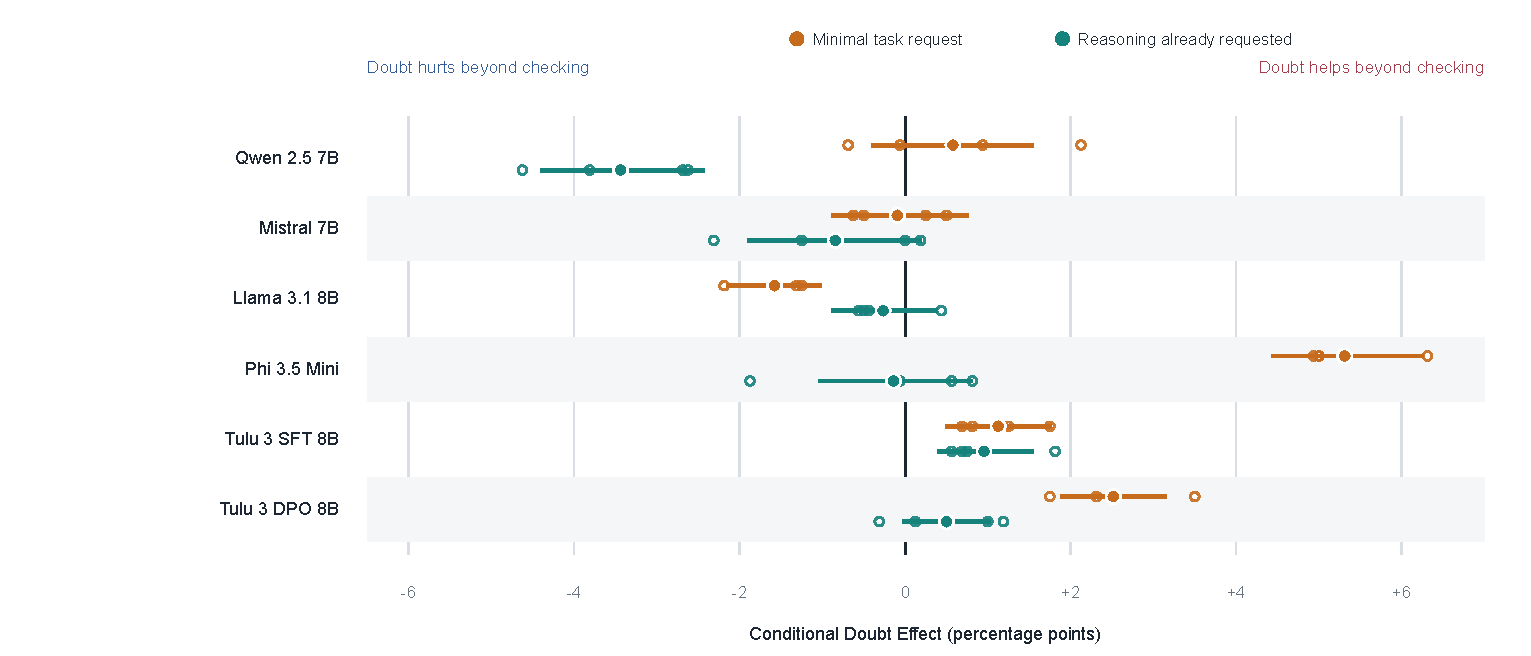
\includegraphics[width=.94\textwidth]{figures/results/cde_context_forest.pdf}
  \color{revisionred}
  \revisioncaptionsetup
  \caption{Conditional Doubt Effect by checkpoint and task context.
  Open circles show the four independent task seeds, filled circles show the
  seed--family macro mean, and horizontal lines are paired 95\% task-bootstrap
  intervals. The sign and magnitude depend on both checkpoint and whether the
  task already requests reasoning.}
  \Description{Conditional Doubt Effect estimates for six checkpoints in minimal and reasoning-requested contexts, showing heterogeneous positive and negative effects.}
  \label{fig:cde-context}
\end{figure*}

\begin{table*}[t]
\centering
\color{revisionred}
\revisioncaptionsetup
\caption{Primary \bench{} scorecard across four task seeds.
Neutral is an accuracy percentage; all other entries are percentage-point
effects. CDE intervals are paired task-bootstrap intervals conditional on the
four prespecified task seeds. Tulu checkpoints share a Llama-3.1 foundation
lineage.}
\label{tab:main-results}
\scriptsize
\begin{tabular}{@{}lrrrrrrr@{}}
\toprule
\textbf{Checkpoint} & $A_N$ & $A_C-A_N$ & \textbf{CDE [95\% CI]} & CDE$_{\min}$ & CDE$_{\mathrm{reason}}$ & \textbf{CM} & $A_{C+Q}-A_C$ \\
\midrule
Qwen 2.5 7B   & 66.44 & +7.70 & $-1.43\;[-2.14,-0.69]$ & +0.58 & -3.44 & -4.02 & -27.05 \\
Mistral 7B    & 24.96 & +0.51 & $-0.47\;[-1.14,+0.20]$ & -0.09 & -0.84 & -0.75 & +1.10 \\
Llama 3.1 8B & 20.00 & +1.45 & $-0.92\;[-1.34,-0.49]$ & -1.58 & -0.27 & +1.31 & -5.63 \\
Phi 3.5 Mini  & 44.98 & +0.45 & $+2.59\;[+1.95,+3.27]$ & +5.31 & -0.14 & -5.45 & -7.53 \\
Tulu 3 SFT 8B & 13.52 & -0.12 & $+1.04\;[+0.60,+1.48]$ & +1.13 & +0.95 & -0.17 & +1.32 \\
Tulu 3 DPO 8B & 16.30 & +1.79 & $+1.51\;[+1.12,+1.92]$ & +2.52 & +0.50 & -2.02 & -3.74 \\
\bottomrule
\end{tabular}
\end{table*}

\subsection{Task-Family and Difficulty Heterogeneity}

\begin{revisionblock}
Aggregate CDE conceals reproducible reversals across the eight task families
(Figure~\ref{fig:family-cde}). Family effects span approximately $-8.4$ to
$+8.9\pp$. For example, Qwen is negative on rule switching ($-8.1\pp$) but
positive on novel-rule learning ($+2.1\pp$); Llama is positive on error
monitoring ($+5.1\pp$) but negative on novel-rule learning ($-8.4\pp$); and
Tulu-SFT reaches $+8.9\pp$ on novel-rule learning but $-4.8\pp$ on goal
management. Twenty-one checkpoint--family effects retain the same nonzero
direction in every seed, making a favorable-generator explanation unlikely.

Difficulty also moderates some effects without defining a universal trend.
Phi rises from $+0.82\pp$ on easy tasks to $+4.49\pp$ on hard tasks, while
Tulu-SFT rises from $-0.39\pp$ to $+2.73\pp$; Qwen and Mistral do not share
this pattern. We therefore treat difficulty as descriptive heterogeneity, not
as a monotonic law.
\end{revisionblock}

\begin{figure*}[t]
  \centering
  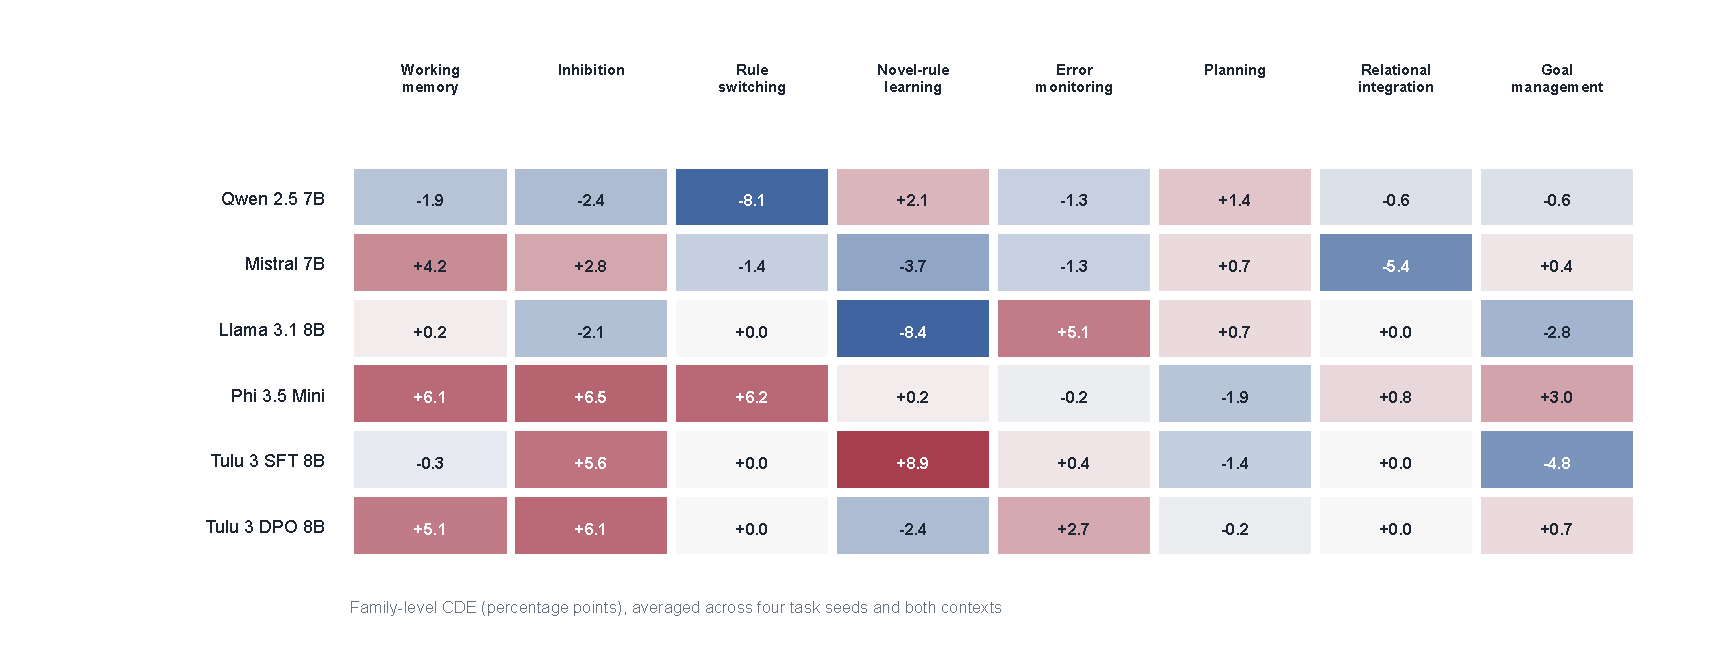
\includegraphics[width=.98\textwidth]{figures/results/family_cde_heatmap.pdf}
  \color{revisionred}
  \revisioncaptionsetup
  \caption{Task-family CDE in percentage points, averaged across
  four task seeds and both task contexts. Aggregate effects hide structured
  reversals: the same prompt component can help one task family and harm
  another for the same checkpoint. Twenty-one checkpoint--family effects
  retain the same nonzero direction in all four task seeds.}
  \Description{Heatmap of Conditional Doubt Effects for six checkpoints and eight task families, showing strong positive and negative heterogeneity.}
  \label{fig:family-cde}
\end{figure*}

\subsection{Seed and Surface Robustness}

\begin{revisionblock}
The family analysis above shows seed-stable directions, but surface wording
still changes exact estimates. Across the 330 latent tasks rendered
canonically, structurally, and as scenarios, mean three-way correctness
agreement is 81.3\%. The median absolute CDE shift from the canonical form is
$1.52\pp$, and only seven of 12 checkpoint--context signs remain invariant
over all renderings (Figure~\ref{fig:surface-cde}). Qwen and Mistral preserve
their minimal-positive/reasoning-negative pattern; several near-zero effects
for Llama, Phi, and Tulu-DPO cross zero. Surface robustness therefore supports
coarse context patterns more strongly than exact effect sizes.
\end{revisionblock}

\begin{figure*}[t]
  \centering
  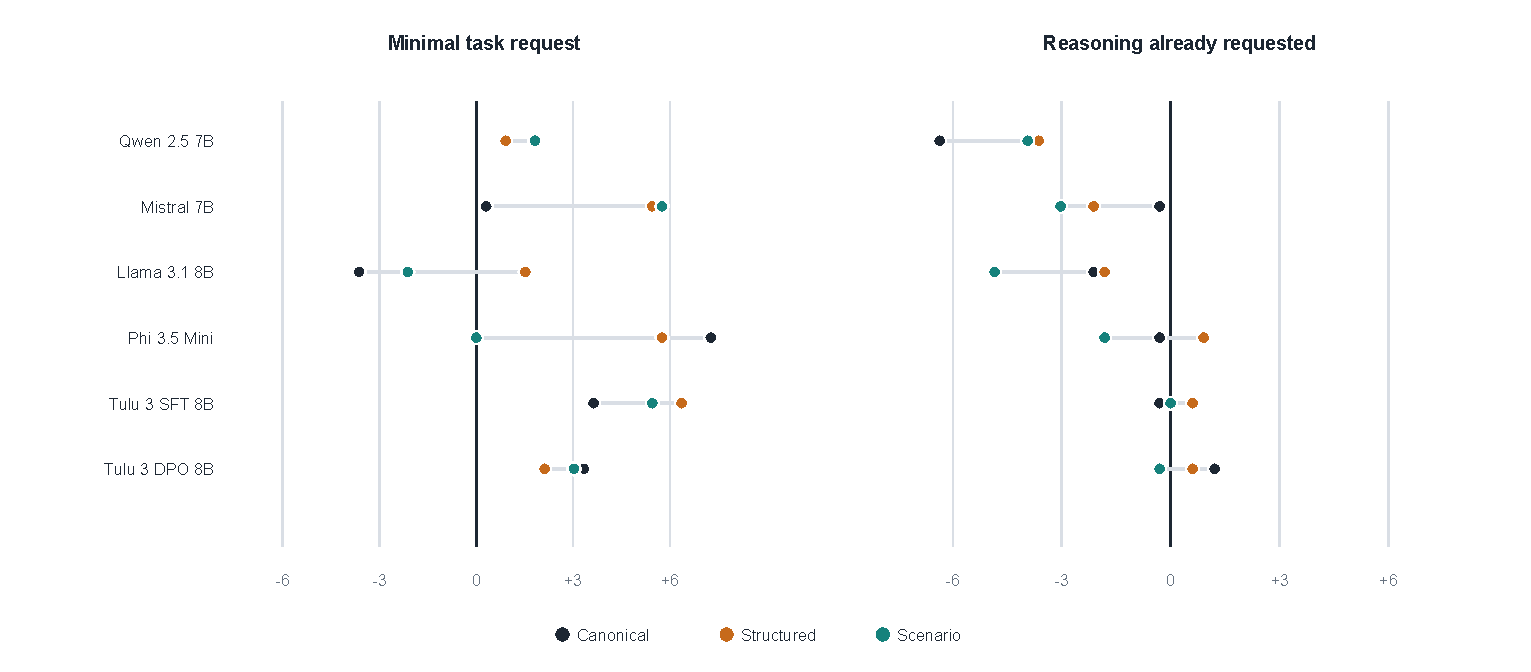
\includegraphics[width=.94\textwidth]{figures/results/surface_cde_robustness.pdf}
  \color{revisionred}
  \revisioncaptionsetup
  \caption{CDE on 330 held-out latent tasks under canonical,
  structured, and scenario renderings. Mean three-way correctness agreement is
  81.3\%, but exact effect sizes move with answer-preserving wording and five
  of 12 checkpoint--context signs cross zero in at least one rendering.}
  \Description{Surface robustness comparison across canonical, structured, and scenario renderings for six checkpoints and two task contexts.}
  \label{fig:surface-cde}
\end{figure*}

\subsection{Post-Training Case Study}

\begin{revisionblock}
Within the shared Tulu/Llama-3.1 lineage, DPO raises neutral accuracy by
$2.78\pp$ and checking gain by $1.91\pp$ relative to SFT
(Table~\ref{tab:tulu-case}). Its overall CDE rises by only $0.47\pp$, but that
average masks a context change: minimal-context CDE increases by $1.39\pp$
while reasoning-context CDE decreases by $0.45\pp$. Post-training therefore
changes prompt sensitivity and context modulation, not merely baseline
competence. This single lineage does not identify a universal effect of DPO.
\end{revisionblock}

\begin{table}[t]
\centering
\color{revisionred}
\revisioncaptionsetup
\caption{Within-lineage Tulu case study. All entries are percentage points;
$\Delta$ is DPO minus SFT. This is not an independent-family comparison.}
\label{tab:tulu-case}
\small
\begin{tabular}{@{}lrrr@{}}
\toprule
\textbf{Endpoint} & \textbf{SFT} & \textbf{DPO} & $\boldsymbol{\Delta}$ \\
\midrule
Neutral accuracy & 13.52 & 16.30 & +2.78 \\
Checking gain & -0.12 & +1.79 & +1.91 \\
CDE$_{\min}$ & +1.13 & +2.52 & +1.39 \\
CDE$_{\mathrm{reason}}$ & +0.95 & +0.50 & -0.45 \\
CM & -0.17 & -2.02 & -1.84 \\
Concision effect & +1.32 & -3.74 & -5.06 \\
\bottomrule
\end{tabular}
\end{table}

\section{Discussion}

\paragraph{Effect existence is not effect attribution.}
A compound prompt can produce a large and reproducible accuracy change while
still failing to establish a self-doubt mechanism. Direct checking is the
relevant control. Conversely, a CDE near zero does not imply that the model
ignored the prompt: wording may alter output length, visible uncertainty, or
format without changing exact correctness.

\paragraph{The benchmark is an experimental instrument.}
\bench{} is designed to estimate controlled prompt effects, not to rank general
reasoning ability or diagnose an internal emotional state. Its usefulness
comes from paired counterfactual structure, fresh exact-answer tasks, and
decomposable endpoints. A later method may use the benchmark to learn when to
apply checking or to normalize compound prompts, but a solver is not required
to make the attribution problem well-defined.

\paragraph{Practical implication.}
\revision{The results reject a universal prompting recipe. Direct checking is
the clearer engineering intervention when it helps, most notably for Qwen,
because it names the desired behavior without anthropomorphic framing. Yet its
gain is small or uncertain for several checkpoints. Self-doubt should likewise
be treated as a model--task-specific intervention: even positive average CDEs
can weaken or reverse when reasoning is already requested.}

\paragraph{\revision{Concision is not free.}}
\revision{The checking-plus-concision condition reduces generated output by a
median 85.4 tokens across the 12 checkpoint--context cells, but its median
accuracy effect is $-3.74\pp$. Qwen under a minimal request loses about 40
accuracy points while emitting roughly 175 fewer tokens. Output length is not
a measure of hidden computation, but this behavioral tradeoff shows why format
compliance and correctness should be reported jointly.}

\section{Limitations and Responsible Use}

The benchmark is procedurally generated and may omit linguistic, domain, and
interaction patterns present in natural user requests. Operational family
labels do not establish equivalence to human cognitive constructs. Exact
scoring favors constrained outputs, while many real tasks require open-ended
judgment. Four foundation families improve breadth but do not represent all
language models, sizes, or post-training procedures. Greedy evaluation does
not quantify model-level sampling stochasticity; the present design instead
targets task and generator variation. Surface variants test limited wording
changes rather than unrestricted paraphrase robustness.

\revision{Five factorial evaluations exceed the prespecified 2\% parse or
truncation threshold: one Qwen seed and all four Llama seeds. The held-out
Llama surface evaluation also exceeds this threshold. Excluding the two
evaluations that combine 384- and 768-token output limits changes overall CDE
by only $+0.02\pp$ for Qwen and $-0.13\pp$ for Llama. A paired
complete-response sensitivity analysis leaves the main Qwen, Phi, and Tulu
patterns intact, but Llama is completion-sensitive: retaining pairs with both
relevant responses moves reasoning-context CDE from $-0.27\pp$ to
$+1.15\pp$. We therefore do not treat Llama's exact effect as a headline
replication. Our conclusions are limited to the controlled task families; we
do not infer transfer to public reasoning benchmarks that lack the matched
five-by-two factorial.}

Prompt interventions are behavioral research instruments. Capability-denial,
emotional manipulation, or sabotage prompts should not be deployed as
user-facing system policies. Released outputs and analyses will avoid claims
that a language model literally experiences doubt or emotion. Benchmark tasks,
scorers, prompt strings, manifests, and raw outputs will be released with
reproducibility documentation, subject to the conference's artifact policy.

\section{Conclusion}

We introduced metacognitive prompt attribution: determining whether
self-doubt language changes task execution beyond the ordinary instruction to
check. \bench{} operationalizes this question with 6,400 latent tasks, eight
families, 33 types, a five-by-two paired factorial, exact scoring, and held-out
seed and surface checks. Its primary endpoint, CDE, isolates the doubt
increment after checking is fixed, while the scorecard preserves competence,
checking gain, context dependence, and robustness. \revision{Across 423,600
responses, CDE is positive for three checkpoints and negative for three, and
only two remain positive after the task already requests reasoning. Large,
seed-stable task-family reversals and measurable surface sensitivity show why
prompt labels and single-domain averages are insufficient for attribution.
Self-doubt language is therefore not a generally reliable correction policy;
it is a conditional behavioral intervention whose incremental value must be
measured against direct checking on the intended model and task.}

\interlinepenalty=10000
\bibliographystyle{ACM-Reference-Format}
\bibliography{references}

\end{document}
